%-----------------------------------------------------------------------------------------
% This template has designed by Mohamad Khaleqi
% You're very welcome to edit and use this template
% 2015-02-26
% Swansea University
%----------------------------------------------------------------------------------------

\documentclass[a4paper,12pt]{article}
\usepackage[utf8]{inputenc}
\usepackage[toc,page]{appendix}

\usepackage{lastpage} % Required to determine the last page for 
\usepackage{graphicx} % Required to insert images
\graphicspath{ {Figs/} }
\usepackage{comment} % Comment
\usepackage[utf8]{inputenc} 
\usepackage{url} % URL in Footnote  
\usepackage{cite} % BibLatex
\usepackage{listings} % hard code
\usepackage[document]{ragged2e} % Justify
\usepackage{wrapfig} % add picture wraped by text
\usepackage{arydshln} % add hash line for tables
\usepackage{booktabs} % new tables

\usepackage{color}
\usepackage{xcolor}
% \newcommand\mytodo[1]{\textcolor{red}{#1}}
\usepackage{lipsum}

\usepackage{tcolorbox} % colour box
\usepackage{float}
\usepackage{courier}
\usepackage{todonotes}
\usepackage{hyperref}
\usepackage{glossaries}
\makeglossaries

\usepackage[nottoc]{tocbibind} % add list of figure and tables and put them in content 

\usepackage[a4paper, margin=1in]{geometry}
\usepackage{pdflscape}

\lstset{frame=tb,
   aboveskip=4mm,
   belowskip=2mm,
   showstringspaces=false,
   columns=flexible,
   basicstyle={\linespread{0.8}\ttfamily\footnotesize},
   numbers=left,
   numbersep=5pt,
   numberstyle=\color{gray},
   keywordstyle=\color{blue},
   commentstyle=\color{dkgreen},
   stringstyle=\color{mauve},
   breaklines=true,
   breakatwhitespace=true
   tabsize=3
}

% Margins
% \topmargin=-0.45in
% \evensidemargin=0in
% \oddsidemargin=0in
% \textwidth=6.5in
% \textheight=9.0in
% \headsep=0.25in 


\linespread{1.3} % Line spacing
\setlength{\parskip}{1em}

%----------------------------------------------------------------------------------------
%	TITLE SECTION
%----------------------------------------------------------------------------------------

%----------------------------------------------------------------------------------------
%	TITLE SECTION
%----------------------------------------------------------------------------------------
\newcommand{\horrule}[1]{\rule{\linewidth}{#1}} % Create horizontal rule command with 1 argument of height
\title{
\begin{Huge}\textbf{RingTMP: Locally Distributed Machine Learning on Low Power Devices} \end{Huge} \\% The assignment title
\vspace{70px}

\includegraphics[width = 65mm]{Figs/SwanseaUniversity.png}\\[8ex]
\begin{large} \textsc{\textbf{Christopher Hopkins}} \end{large} \\ % Your university, school and/or department name(s)
\vspace{10px}
\normalfont \normalsize 
\begin{normalsize}Department of Computer Science \end{normalsize}\\  % Your university, school and/or department name(s)
\begin{normalsize} Swansea University \end{normalsize} \\ % Your university, school and/or department name(s)
\vspace{60px}
This dissertation is submitted for the degree of\\
\textit{Bachelor}
\vspace{20px}
}


%------------------------------------------------------------------------------------
% Document begin
%------------------------------------------------------------------------------------
\begin{document}
\pagenumbering{gobble} %stop page number
%------------------------------------------------------------------------------------
% Page Title
%------------------------------------------------------------------------------------
\begin{titlepage}

\maketitle
\vfill
% \center \date{\normalsize October 2020} % Today's date or a custom date
\end{titlepage}
% -----------------------------------------------------------------------------------

\pagenumbering{Roman} 
\justify
% ******************************* Thesis Declaration ***************************
\null\vspace{\fill}
\renewcommand{\abstractname}{\large Declaration}
\begin{abstract}
\vspace{2cm}

This work has not been previously accepted in substance for any degree and is
not being con-currently submitted in candidature for any degree. This thesis is
the result of my own investigations, except where otherwise stated. Other
sources are acknowledged by footnotes giving explicit references. A bibliography
is appended. I hereby give my consent for my thesis, if accepted, to be made
available for photocopying and inter-library loan, and for the title and summary
to be made available to outside organisations.

\vspace{1cm}
\begin{flushright}
 Christopher Hopkins\\
 October 2020
\end{flushright}

\end{abstract}

\vspace{\fill}
% ************************** Thesis Abstract *****************************
\null\vspace{\fill}
\renewcommand{\abstractname}{\large Abstract}
\begin{abstract}
\vspace{2cm}

% More data than ever is being produced by low power devices such as smart phones
% and Internet of Things (IoT) devices at the network edge. The data being
% produced is so enormous it would be infeasible to send it to a centralised
% location. Instead models can be trained from data distributed across multiple
% edge nodes, with machine learning algorithms being performed locally. In this
% paper I explore training multiple low power devices using a new distributed
% machine learning paradigm \textit{RingTMP}. This paradigm focuses  on low power usage
% and power efficiency while having the capacity for larger models than
% comparative systems.

There is no argument that large scale datasets have never been more available
than they are now. Naturally, machine learning algorithms have been applied to
these datasets to derive useful information from them. Machine learning models
have scaled with the data. Our machines have scaled too, using distributed
frameworks such as parameter servers in order to complete machine learning tasks
in a feasible amount of time. However our current methods are reaching their
limits, as the communication between distributed nodes can overwhelm the limited
bandwidth between them.

This paper describes a novel paradigm for distributed machine learning
\textit{RingTMP}. This ring topological model parallel neural networking
framework aims to reduce the amount of communication between nodes, while still
training just as fast and as accurately as a generic comparative parameter
server. This framework along with a non distributed neural network and a generic
parameter server is trained on the Iris and MNIST numbers datasets. The results
show that RingTMP converges at least as fast as the parameter server, while in
some tests dramatically reducing data transmission as much as 380x per epoch and
as much as 8x per unit time.

\end{abstract}
\vspace{\fill}


%------------------------------------------------------------------------------------
% Table of content
%------------------------------------------------------------------------------------
\tableofcontents
\pagebreak
% \listoffigures
% \pagebreak
% \listoftables
\justify
%------------------------------------------------------------------------------------
% Document begin
%------------------------------------------------------------------------------------
\clearpage
\pagenumbering{arabic}
%-----------------------------------------------------------------------------------------

\section{Introduction}
%-----------------------------------------------------------------------------------------

\subsection{Motivation and Context}

Machine Learning has become an invisible but ubiquitous part of modern life, and
is being used in a plethora of fields and industries. The uses of this
technology range from dystopian facial recognition
\cite{mattBurgessFacialRecognision} to lifesaving diagnoses
\cite{Mammograms2020} and many more purposes besides. Machine Learning leverages
existing data to train Machine Learning models in order to perform a task or
find patterns, that previously only a human could. The key difference between
Machine Learning and conventional programs is that the data itself is used to
develop the model. Therefore the quality and quantity of the data can affect the
effectiveness of a machine learning model.
\par
As the amount and complexity of the data we are collecting increases so does the
size and complexity of the machine learning models we use to make sense of our
data. For example the internet archive as of 2020 contains over 70 petabytes of
data, while labeled datasets such as AViD have video data in the order of
terabytes. \cite{piergiovanni2020avid} We are now reaching a point where the
limiting factor of creating a machine learning model is not the data, but the
machine learning algorithm itself.
\par
This problem is two pronged. First machine learning models are getting very,
very large. For instance GPT-3 the largest Natural Language Model ever trained
contains 175 billion parameters. \cite{fewshowlearners2020gpt} And efforts are
being made to create models with trillions of parameters.
\cite{rajbhandari2020zero} We have reached the point where its no longer
possible to store some machine learning models on a single
machine.\cite{LI2014ParameterServers}
The second problem is that training a machine learning model is increasingly
taking longer and longer. This is because we have more data and larger models,
but the algorithms used to train models have fundamentally stayed the same and
are inherently sequential and difficult to parallelise.
\par
The popular current solution is to use a parameter server model. In brief the
paradigm is made of two different types of components. The parameter server and
the workers. The parameter server holds the global parameters of the model.
Workers are given the model parameters by the parameter server. The workers then
perform an iteration of whichever machine learning algorithm they are
performing, modifying the parameters. Then the modified parameters are sent to
the parameter server where they are aggregated, the global model parameters are
updated and the cycle continues until the model has converged on an answer.
However this method has two key drawbacks. First, every worker must communicate
with a single parameter server, this limits scalability as eventually the
network bandwidth becomes saturated severely impacting performance.
\cite{LI2014ParameterServers} Secondly many parameter server models require the
whole model to be replicated within each node. \cite{jia2018BeyondData} This
means that very large models simply cannot run on many machines.
\par
In this paper I will outline an alternative distributed machine learning
framework: \textit{RingTMP}. RingTMP (Ring Topological Model Parallel) is a Ring
Topological Model Parallel distributed machine learning framework focusing on
optimising Distributed Gradient Descent. This is a novel design drawing in
inspiration much research but particularly from the STRADS and DistBelief
machine learning frameworks. \cite{kim2016STRADS,Dean2012Distbelief}
\par
I believe my distributed framework may have some advantages over the current
paradigm, these briefly are:
\begin{itemize}
    \item There will be less communication between nodes
    \item A Potential for larger communication bandwidth between nodes
    \item My framework will be able to hold larger models
    \item Will be able to train neural networking models as faster or faster
    than a comparative parameter server, to the same level of accuracy
\end{itemize}

My aims more specifically for this project are to:
\begin{itemize}
    \item Create a prototype RingTMP framework.
    \item Create a parameter server model framework.
    \item Demonstrate less communication between nodes
    \item Demonstrate that RingTMP is at least as scalable than a generic parameter
    server.
    \item Demonstrate that RingTMP can hold larger models on comparison to a
    standard parameter server.
    \item Demonstrate RingTMP can train Neural Networks to at least the same
    accuracy in at least the same amount of time.
\end{itemize}


% Should do power consumption if I have enough time
% \item Demonstrate that RingTMP takes less overall power to run in comparison
% to the parameter server.




% %-----------------------------------------------------------------------------------------
\clearpage
\section{Related Works}
%-----------------------------------------------------------------------------------------


%-----------------------------------------------------------------------------------------
\clearpage
\section{Literature Review}
%-----------------------------------------------------------------------------------------
\subsection{Brief Introduction to Machine Learning and Neural Networks}
To first understand distributed machine learning you must first understand the
fundamentals of machine learning and neural networks. There are many machine
learning methods some requiring training data which we call supervised and some
being able to find patterns in data without being given solutions called
unsupervised. \cite{alpaydin2020introduction} Neural networks tend to focus on
supervised learning and use a form gradient descent called stochastic gradient
descent.

Many machine learning algorithms use a cost function to measure how well or
badly they are solving a problem, these algorithms use parameters which are
internal variables of a machine learning model and define how they solve the
problem. If you map \(costFunction(x)\), where \(x\) is the model parameter, for
every \(x\) value. Then a graph will be produced \(y = costFunction(x)\), the
lowest point on the graph will be the global minimum. There may be other troughs
higher than the global minimum these are called local minimums. A global minimum
represents the lowest value of the cost function which indicates the parameter
values produce the best solution for your problem. Initial model parameters are
often randomised, which likely means they will start at a high point on the cost
function graph, the goal is to get to the lowest point possible. To do this you
must \textit{descend} down the \textit{gradient} to a local minima, the
algorithm that does this is called gradient descent for that very reason. This
often happens in little steps after the observation of each piece of data.
However it is computationally expensive to step down the gradient after each
example. It is more efficient to calculate the average step of a randomised
selection of data. This is know as stochastic gradient descent.

Neural networks are structures that can perform multi-variable gradient descent
when provided with training data. They are comprised of layers of
interconnected neurons in a lattice like structure. Each neuron holds parameter
information the adjusting of which through gradient descent leads to the solving
of a problem through reaching the local minimum of the cost function.

\subsection{Limited History of Distributed Machine Learning}


One of the first instances of distributed machine learning was used to
categorise New York Times articles using Latent Dirichlet Allocation (LDA),
which identifies the affiliations words have to certain topics.
\cite{newman2008distributed} While the paper focused on parallelising the
algorithm and running them over multiple artificially isolated cores the results
showed that distributed machine learning could have scalability and didn’t
impact the rate of convergence of the model significantly. This was followed by
a paper by Jia et al. \cite{ParallelTopicModels} which produced much faster
results than its predecessors by using memcache layer in every machine, every
machine would message every other with updates of its local parameters
to create an approximate global state, it was mentioned in passing that
arranging the nodes in a star topology and caching the values that passed
through it could make the system more scalable. After this followed a cambrian
explosion of work in this area \cite{Ahmed2012YahooLDA, li2014communication,
Dean2012Distbelief, googlemapreduce2008} culminating in 2014 when the parameter
server as it is known today \cite{LI2014ParameterServers} was produced.


\subsection{Model and Data Parallelism}
\begin{figure}[h]
    \centering
    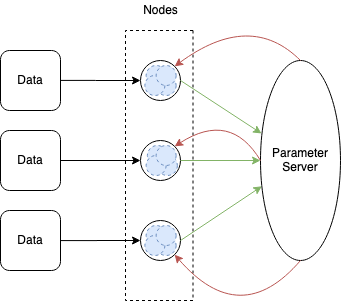
\includegraphics[width=0.4\textwidth]{DataParallel}
    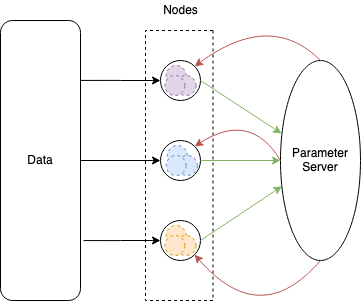
\includegraphics[width=0.4\textwidth]{ModelParallel}
    \caption{Left: Data Parallelism. Right: Model Parallelism. In both diagrams
        the green lines indicate local parameters being sent to the parameter
        server and red lines indicate parameters being sent to the worker nodes.}
\end{figure}
When creating distributed machine learning models there are two different methods
for distributing training, model parallelism and data parallelism. These two
methods are not mutually exclusive and can be used in conjunction with one
another, such as in DistBelief. \cite{Dean2012Distbelief}. Model parallelism is
when model parameters are split between the nodes. As data parallelism is when
the training data is split between the nodes. \cite{Xing2015Petuum} Often with model
parallelism the whole set of training data is passed through each node. While in
data parallelism its common for each node to hold the whole machine learning
model.

The key advantage of model parallelism is that machine learning models can be
far larger as they no longer have to train the whole model on one machine.
However this one great advantage comes with some disadvantages. Some parameters
may take more time to converge than others, this means that at times some nodes
may be idle while others are still converging, so the spread of computation is
not equal or efficient. \cite{Dean2012Distbelief} Because some parameters
converge at different rates a scheduler can be used, which does improve model
convergence. However this requires more computational overhead and communication
while reducing iteration throughput.
\cite{kim2016STRADS}

Data parallelism has the benefit that data throughput can be very large, making
processing using this method fast. However with more nodes, the
communication overhead increases as the nodes must communicate the changes in
their model parameters to the parameter server. \cite{elgabli2020gadmm}

\subsection{Model Consistency}
Both of these parallel paradigms still function on the basis of a strictly
iterative model, where communication is the limiting factor. Creating a generic
parameter server similar to how Googles map reduce algorithm is implemented
\cite{googlemapreduce2008} is still in some sense sequential. The next iteration
can't continue until all workers have responded with their updated parameters,
and each worker must send its results back no matter how significant its work
is. Relaxing these restraints in specific ways have been shown to produce faster
training times, while still converging on a model just as accurate. Especially
when time, not data is at a premium.\cite{li2014communication}
\par
Partially relaxing the iterative restraint of the parameter server and instead
using a bounded delay, dramatically decreases the wait times of workers to
almost 0. A bounded delay allows workers to operate on slightly stale
parameters. Unintuitively this allows for faster convergence than the sequential
model, as it can iterate over the data faster and learn almost as much from each
iteration. \cite{li2014communication}.
\par
The other restraint that can be relaxed is the requirement to always send
updated weights back to the parameter server. Many training examples don't
dramatically change the parameters. Therefore only the training examples that
cause the parameters to change significantly need to be sent back to the
parameter server. This also allows for greater scalability, as each worker only
communicates significant updates to the parameter server, meaning more nodes can
be used before saturating the network. \cite{li2014communication}. 

\subsection{The Communication Issue}
% TODO: EXPAND by talking about the magnitudes in speed between local training
% and training via nodes? 


Distributed neural networks must communicate with each other in some way in
order to work together. This needs to be formalised to be able to measure the
efficiency of our machine learning system. Parts of this reasoning already
appears in these papers too. \cite{konevcny2016federated ,Ma2017DistributedOptimisation}

If we consider how a neural network operates if we were to run it on a single
node, we could characterise its computation as such:
\begin{equation}
    TIME = I_A (\epsilon) \times T_A 
\end{equation}

Where \(I_A(\epsilon)\) is the number of iterations of the algorithm \(A\) it
takes to reach accuracy \(\epsilon\) and \(T_A\) is the time of each iteration
of the algorithm. Here maximising the convergence per iteration or decreasing
the time an iteration takes will decrease the runtime of the algorithm. In a
distributed setting this equation changes to this:
\begin{equation}
    TIME = I_A (\epsilon) \times (c + T_A)  
\end{equation}
In this equation we have the added variable \(c\), this represents time taken
for communication per iteration. In a distributed setting this will always
remain above a non trivial amount of data. Unfortunately the majority of machine
learning algorithms use a stochastic method which means a very large number of
iterations \((I_A(\epsilon))\) that take a short amount of time (small \(T_A\)).
You can see that no matter how small \(c\) is there will be a significant impact
of the time taken. In fact with a naive approach of communication \(c > T_A\) is
almost certainly true for each iteration.

However this view doesn't take into account the possibility that communication
could happen at the same time as an iteration. For example imagine a pipeline of
nodes where each nodes performs an iteration but can communicate its previous
iteration to the next node at the same time. Then the time taken could be
described like so:
\begin{equation}
    TIME = I_A (\epsilon) \times max(c, T_A)
\end{equation}
Here you can see that if you can find a way of making the communication time
equal to the time per iteration. Then \(c\) would have a negligible effect on
the equation.


% Do I need to include this?
\subsection{Low Power Hardware, IoT and Mobile Computation}

Historically machine learning algorithms have been focused on high model
accuracy through large models and vast amounts of training data, energy
consumption and efficiency has rarely been taken into consideration. However
with the rise of Internet of Things (IoT) devices and the established ubiquity
of smart phones more data than ever is being produced. Soon this data generation
will exceed the capacity of the internet, and experts estimate that over 90\% of
data will be stored and processed locally. \cite{Chaing2016FogIoT} By extension
this means machine learning algorithms will have to be performed locally too.
This introduces some challenging issues. Modern machine learning algorithms
require vast centralised computational power and large amounts of data. Local
devices don't have the capacity to hold large data sets or the power to compute
large machine learning models in a viable amount of time, while many of them are
also battery powered so power consumption becomes another issue.

% modern solutions for edge computing 
A solution to this is to massively distribute the model over multiple
decentralised nodes. The level of distribution is even greater than that of
centralised compute clusters. In this solution each device computes a model
using its own local data, infrequently (due to network constraints) the model is
shared with a coordination server, which will then distribute the changes across
all nodes in the network. \cite{wang2018EdgeLearning} While this method is
inefficient as the infrequent communications mean that many nodes may do much of
the same work, and the merging of local models into a global one infrequently
may cause loss of information. It still produces a model which converges in a
relatively few rounds of communication. \cite{konevcny2016federated}

% low power solutions
Efforts have been made in techniques to reduce the power memory and storage
needed for machine learning algorithms to operate. One of these is Data Stream
Mining. The idea is that a device can stream the analytics data directly into
the model rather than storing the data in storage for later use.
\cite{garciaMartin2019MLEnergy} This means after the data has been read by the
model it is lost. But that also means that no data needs to be stored, meaning
resources are not spent reading and writing to storage. This has an application
in mobile devices, as they produce data at a low rate through user interaction.
Therefore the model can be build in real time as actions occur. The data
produced on the mobile itself may not be enough to effectively train the model,
but via communication with other users distributed over the network the model
can converge. \cite{konevcny2016federated}


%-----------------------------------------------------------------------------------------
\clearpage
\section{Problem Description}
%-----------------------------------------------------------------------------------------xs

% show the ideal situation
In the most ideal world, communication between distributed network nodes would
not to bottleneck performance. As many nodes as you liked could be added to your
network and performance would scale linearly with each node added.


% In the most ideal world, communication between distributed network nodes would
% never saturate bandwidth and each node would spend all of its time on
% computation rather than waiting. This would enable distributed machine learning
% to iterate just as fast as single node machine learning.

% show the situation as it currently exists
Currently when distributed neural networks become large enough, they become
saturated. Adding more nodes no longer increases the speed of computation. To
increase the speed of training further by adding more nodes at least one of two
things must happen. Either the bandwidth between each node must be increased or
the nodes must communicate less while still communicating enough information to
continue training.\cite{li2014communication}\cite{SunTimeDataflow} This limit in
the rate of computation means that training a neural network cost more time and
money. We are at the point now where even if mistakes are found in the largest
projects, its often 'infeasible' to retrain the model due to time and monetary
cost. \cite{fewshowlearners2020gpt}

% Ultimately we want to make neural networks faster to train. The way this is
% achieved from the perspective of distributed neural networks is to create more
% neural network nodes. The communication between nodes often saturates the
% network, when this happens adding more nodes no longer speeds up computation.
% \cite{li2014communication}. To increase the speed of training further by adding
% more nodes at least one of two things must happen. Either the bandwidth between
% each node must be increased or the nodes must communicate less while still
% communicating enough information to continue
% training.\cite{li2014communication}\cite{SunTimeDataflow}
% cite 
% \par
% Training a neural network model is not deterministic, it often takes multiple
% attempts and adjustments to train. Even when the model is training with some
% stability it can take many attempts to produce the most accurate model. This
% takes enormous amounts of time and processing power. Reducing the amount of time
% and by extension the cost of training would mean that researchers and developers
% would be able to iterate on there models faster accelerating the rate at which
% the field itself develops. Even in situations where researchers have the most
% resources, when mistakes are made its often 'infeasible' to retrain the model
% due to time and monetary cost. \cite{fewshowlearners2020gpt}
\par
% the consequences if this is ignored
The impact of leaving this problem unsolved will mean the limiting factor of
distributed neural networking will be not the processing power of the nodes but
the bandwidth between them, bandwidth being one of the scarcest resources in
data centres \cite{LuizDatacenterAsAComputer}. It will stifle the growth of
machine learning models, especially for those that cannot get the funding for high
bandwidth compute clusters.

This is why I designed a new paradigm for distributed neural networking that
should reduce the communication between each node relative to a generic
parameter server. The new paradigm also allows for higher bandwidth between
adjacent nodes. As in this scenario nodes need only communicate with their
adjacent partner. This results in a distributed learning model that isn't bound
by bandwidth when scaling, and should be able to train models to the same level
of accuracy in the same amount of time.

% The impact of leaving this problem unsolved will place
% a semi-hard limit on the scalability of distributed machine learning. Bandwidth
% being one of the scarcest resources in data centers, up to 100 times smaller
% than local memory bandwidth. \cite{LuizDatacenterAsAComputer} Distributed
% machine learning speed will be limited by t

% add some more evidence with citation here
% less communication bandwidth you can cite significant update thing, or compressing
% carnigie mellon university did some work with globe distributed machine learning, look that up


% As it stands bandwidth is the factor limiting how many
% nodes a distributed neural network can scale to. This in turn 

% the consequences of not solving the problem


% Bandwidth restrictions between nodes place a limit
% Through reading the relevant literature, the key problem of this project is this. How can we optimise communication between workers




%-----------------------------------------------------------------------------------------
\clearpage
\section{Implementation}
%-----------------------------------------------------------------------------------------

\subsection{Tooling}
Implementing a distributed neural network is too large a task to be undertaken
from scratch. Therefore its necessary to used existing tools, to make the
development viable in the time given. This is difficult as not many languages
lend themselves to both distributed systems and neural networks.

To ensure high performance the project could be implemented in C++. While C++ is
often very performant and also has low level bindings for ML libraries such as
TensorFlow. However even the creator of the language sees the need to improve
its ability to improve its distributed performance. \cite{stroustrupInterview}

Python has great tooling for neural networking, such as TensorFlow
\cite{abadi2016tensorflow}, and PyTorch \cite{paszke2019pytorch}. Moreover it
has great support for numerical computing with NumPy \cite{harrisNumpy2020}.
These are performant too, by calling C functions or creating code which is
optimised to run on GPUs to parallelise computation. However due to the Global
Interpreter Lock (GIL) python is infamously bad at concurrency, while its
distributed tooling is implemented in native python code, which lack of speed
and could bottleneck the performance gained from using NumPy and TensorFlow.

Ultimately I decided to use Elixir as the programming language of
implementation. This is because Elixir was designed for developing highly
concurrent distributed systems. It does this by having a uniquely brilliant
concurrency model. As opposed to OOP languages where 'everything is an object'
in Elixir 'everything is a process'. This means the default way of writing the
language enables it to be concurrent and scalable. Elixir also has the ability
to communicate with other Elixir programs over the network using its own
application protocol on top of TCP/IP. Meaning its as easy to communicate with
local processes on your own machine as processes on another machine running an
Elixir program. Its also been used by artificial intelligence researchers before
as the process concurrency models effortlessly lends itself to modelling
neurons. \cite{sherNeuroevolutionThroughErlang} Using Elixirs native float and
arithmetic implementation would be slower than a C++ or a NumPy implementation,
luckily there is a stable package which supports matrix calculations even faster
than those in NumPy called Matrex. \cite{matrex}

The only drawback of using Elixir is at the time of development it didn't have a
strong machine learning library, which means implementing the mathematics of the
neural network myself. While this was a sizeable amount of work to do, it had
the benefit that I didn't to wrestle with an opinionated API such as TensorFlow,
I could create my own API to meet my ends.

\subsection{Neural Network Implementation}
In order to create a distributed neural network. I first needed to create a
basic feed forward network that could operate on a single machine. This network
didn't need to be fully featured, its just a means to make an objectively
comparative performance between RingTMP and a generic parameter server.
Therefore only 2 types of layers were implemented, the hidden layer and the
output layer. The hidden layer is a generic dense layer similar to the kind you
would find in any other neural network library. The output layer performs
similarly to the hidden layer with the key difference that its always the final
layer and outputs the activations as probabilities. Within this section I will
explain in more detail how the neural network was implemented from scratch and
the mathematics behind its function.

% creating a network should go here first
\subsubsection{Initialisation}
Neural networks are composed of layers, while conceptually layers are
composed of neurons, they're practically implemented with two components. A
weights matrix and a bias vector. As I have already mentioned in this network
there are two types of layers, hidden layers and output layers. We need to label
each layer with its type, so we know how to perform the forward and
backpropagation. Therefore we can describe a layer as the tuple:
\begin{lstlisting}[numbers=none,frame=none]
    {layer_type, weights, bias}
\end{lstlisting}

Placing several of these tuples in a list creates a network:
\begin{lstlisting}[numbers=none,frame=none]
  [{:hidden_layer, weights_1, bias_1},
   {:hidden_layer, weights_2, bias_2},
   {:output_layer, weights_3, bias_3}]
\end{lstlisting}

The weights and biases have different dimensions depending on the layers input size
and output size. A layer might take an activations vector with a size of \(m\) and
output a size of \(n\). The layer would hold a \(n \times m\) matrix
and the dimensions of the bias would be \(n \times 1\). The
output size of one layer must be the input size of the next layer, else the
network will fail to function.

Initialising the biases is simple, as biases have the function of an intercept
in a linear equation, they can be initialised to 0. The trivial code is below:
\begin{lstlisting}
  defp initialise_bias(col) do
    Matrex.zeros(col, 1)
  end
  \end{lstlisting} 

Weights are more complex. Each layer is initialised with random values from a
uniform distribution, the shape of the uniform distribution is dependant upon
the size of the input and output layers of the neural network. The type of
initialisation used is dependant upon the activation function used.

In the hidden layer the ReLU function is used, common wisdom first established
in this paper \cite{he2015delving} states that for the fastest convergence He
initialisation should be used. He initialisation is done by sampling random
values from a normal distribution with a mean of 0 and a variance of \( 2/N \)
where \(N\) represents the number of input values to a layer.

For the output layer, the softmax function is used. The best initialisation
method in this case is using Xavier
initialisation. \cite{glorot2010understanding} This also takes random samples
from a normal distribution with a mean of 0 but has the variance of \( 1/N \)
where \(N\) is \( (inputSize + outputSize) / 2 \).

However in practice training the model often failed with He initialisations.
This was because of what is know as the 'Dying ReLU Problem'. Which is when the
elements of the z vector of a layer are negative, the ReLU activation function
will return a zero meaning no learning is taking place. Once a neuron becomes
dead its unlikely it will be revived as the function is piecewise and provides
no slope for recovery such as a Leaky ReLU or a sigmoid function. To remedy this
I trialed many distributions, settling on a mean of 0.5 with a variance of 0.25.
While this is more simplistic, and may impact training times, its far more
likely for the network to not be dead on arrival because of the initialisation
parameters. This is part of the code which initialises the matrices in the layers:
\begin{lstlisting}
  defp random_val(_x, {n, :he, seed_state, acc}) do
    {val, new_state} = :rand.normal_s(0, 2 / col, seed_state)
    {col, :he, new_state, [val | acc]}
  end

  defp random_val(_x, {n, :pos, seed_state, acc}) do
    {val, new_state} = :rand.normal_s(0.5, 0.25, seed_state)
    {n, :pos, new_state, [val | acc]}
  end

  defp random_val(_x, {n, :xavier, seed_state, acc}) do
    {val, new_state} = :rand.normal_s(0, 1 / col, seed_state)
    {col, :xavier, new_state, [val | acc]}
  end
\end{lstlisting}

you can find the wider context for this code snippet in code listing in the Appendix 1. ~\ref{network_initialisation} 

\subsubsection{Forward Propagation}

% need to put this stuff earlier its already been explained
Neural networks are composed of layers, each layer is composed of neurons.
Numerical inputs are inserted through the input layer, forward propagate through
the network and push numerical results to the output layer. For our purposes
each neuron in the output layer represents a different category, the value of
that neuron is the probability the given input belongs to that category.

Each neuron holds a value, called an activation. Each layer has a bias and a
collection of neurons. Between the layers every neuron in one layer connects to
every other neuron in the next layer, every connection has an associated value
called a weight. To calculate the weight of a single neuron in the next layer
you must multiply the activations of the previous layer with the weights
connected to the neuron in question, then sum the values, add the bias, then
apply the activation function to that value. To explain more visually the
process and mathematics more visually, see the diagram below of the interaction
between two layers each with two nodes.

<<REDO THIS BIT ABOVE>>

\begin{figure}[h]
    \centering
    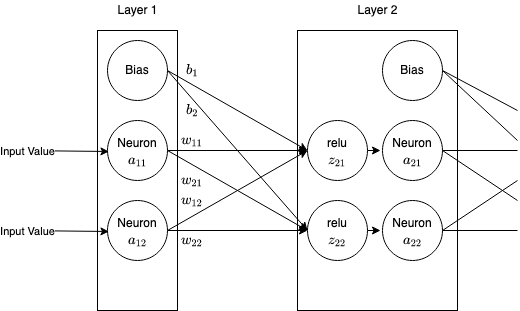
\includegraphics[width=0.6\textwidth]{two_neuron_network_1}
\end{figure}

\begin{equation}
    \begin{aligned}
        z_{21} &= a_{11}w_{11} + a_{12}w_{12} + b_{1} \, \, \, \, \, \, \, z_{22} = a_{11}w_{21} + a_{12}w_{22} + b_{2} \\
        a_{21} &= relu(z_{21}) \, \, \, \, \, \, \, a_{22} = relu(z_{22}) 
    \end{aligned}
\end{equation}


As networks become larger using this notation above becomes cumbersome. So we
use matrices to simplify the situation. Where \(X\) is the input matrix, \(W\)
is the weights, \(B\) is the bias, \(activationFunc(x)\) is the activation function and finally \(A\) is the output activation.

\begin{equation}
    \begin{aligned}
        X = \begin{bmatrix}
            a_{11} \\
            a_{12}
        \end{bmatrix} \, \, \, \, \, \, \,
        W &= \begin{bmatrix}
            w_{11} & w_{12} \\
            w_{21} & w_{22}
        \end{bmatrix} \, \, \, \, \, \, \,
        B = \begin{bmatrix}
            b_{1} \\
            b_{2}
        \end{bmatrix} \\[10pt]
        A &= activationFunc( W^{T}X + B)
    \end{aligned}
\end{equation}

In my implementation there are only two layer types. Hidden layers and output
layers. The only difference between these two layers is the activation function
that they use. Hidden layers use the ReLU activation function which is a simple
piecewise non-linear function described as such:
\begin{equation}
    relu(z) = max(0,z)
\end{equation}
This function has become the de facto application function in dense hidden
layers since its debut in 2011. \cite{glorot2011deep}. In Elixir the forward
action in the hidden layer is implemented like so: \footnote{The pipe operator
\lstinline{|>} transforms the function \lstinline{val_a |> a_function(val_b)}
into \lstinline{a_function(val_a, val_b)}}
\begin{lstlisting}
  def forward(previous_activation, weights, bias) do
    weights|> Matrex.transpose()
    |> Matrex.dot(previous_activation)
    |> Matrex.add(bias)
    |> relu()
  end

  defp relu(z_vector) do
    z_vector|> Matrex.apply(
        fn value, _index -> if value > 0, do: value, else: 0 end
    )
  end
\end{lstlisting}

The output layer uses a more complex activation function, the softmax function,
which transforms its inputs into probabilities. The sum of these probabilities
is always 1. This is the softmax function, where \(z\) is a \(i \times 1\)
vector:
\begin{equation}
    softmax(z)_{i} = \frac{e^{z_{i}}}{\sum_{j=1}^{n} e^{z_{j}}}
\end{equation}

This function is implemented the categorical output layer like so:
\begin{lstlisting}
    def forward(previous_activation, weights, bias) do
        weights|> Matrex.transpose()
        |> Matrex.dot(previous_activation)
        |> Matrex.add(bias)
        |> softmax()
    end

    defp softmax(z_vector) do
        stabilised_vec = Matrex.subtract(z_vector, Matrex.max(z_vector))
        exp = Matrex.apply(stabilised_vec, :exp)
        Matrex.divide(exp, Matrex.sum(exp))
    end
\end{lstlisting}

% show forward propagation function across the networks





% put equations here

% second diagram here
% second equations here

% $$a_{2} = relu(z)$$

% $$z = a_{1}w + b$$

% \begin{figure}[h]
%     \centering
%     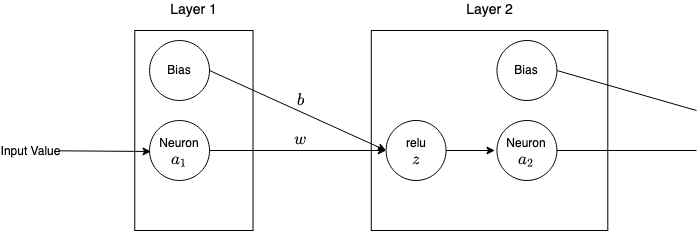
\includegraphics[width=0.6\textwidth]{simplest_neural_network_1}
% \end{figure}
% \begin{equation}
%     z_{21} = a_{11}w_{11} + a_{12}w_{12} + b_{1} \, \, \, \, \, \, \, z_{22} = a_{11}w_{21} + a_{12}w_{22} + b_{2}
% \end{equation}
% \begin{equation}
%     a_{21} = relu(z_{21}) \, \, \, \, \, \, \, a_{22} = relu(z_{22}) 
% \end{equation} 
% \begin{equation}
%     z = a_{1}w + b
% \end{equation}
% \begin{equation}
%     a_{2} = relu(z)
% \end{equation}

% The activation function being used
% in the hidden layers in this project is the ReLU function, which has become the de
% facto activation function since its discovery in 2011. \cite{glorot2011deep}

%-----------------------------------------------------------------------------------------
\clearpage
\section{Requirement and Specification}
%-----------------------------------------------------------------------------------------
\subsection{Keywords}
\begin{table}[ht]
\centering

\begin{tabular}{ll}
\toprule
Keyword  & Definition \\

\midrule
Completed & The requirement is implemented or fulfilled \\
Partial & The requirement is partially implemented or fulfilled \\
Not Completed & The requirement is not implemented or fulfilled \\
FR & Functional Requirement \\
NFR & Non Functional Requirement \\
FS & Functional Specification \\
NFS & Non Functional Specification\\

\bottomrule

\end{tabular}
\caption{Keywords} \label{tbl:keywords}
\end{table}

\subsection{Requirements}
\lipsum[2]

\subsection{Specification}
\lipsum[1]

\subsection{Cross-References} 

\lipsum[5-7]
% %-----------------------------------------------------------------------------------------
\clearpage
\section{Implementation}
%-----------------------------------------------------------------------------------------

\subsection{Tooling}
Implementing a distributed neural network is too large a task to be undertaken
from scratch. Therefore its necessary to used existing tools, to make the
development viable in the time given. This is difficult as not many languages
lend themselves to both distributed systems and neural networks.

To ensure high performance the project could be implemented in C++. While C++ is
often very performant and also has low level bindings for ML libraries such as
TensorFlow. However even the creator of the language sees the need to improve
its ability to improve its distributed performance. \cite{stroustrupInterview}

Python has great tooling for neural networking, such as TensorFlow
\cite{abadi2016tensorflow}, and PyTorch \cite{paszke2019pytorch}. Moreover it
has great support for numerical computing with NumPy \cite{harrisNumpy2020}.
These are performant too, by calling C functions or creating code which is
optimised to run on GPUs to parallelise computation. However due to the Global
Interpreter Lock (GIL) python is infamously bad at concurrency, while its
distributed tooling is implemented in native python code, which lack of speed
and could bottleneck the performance gained from using NumPy and TensorFlow.

Ultimately I decided to use Elixir as the programming language of
implementation. This is because Elixir was designed for developing highly
concurrent distributed systems. It does this by having a uniquely brilliant
concurrency model. As opposed to OOP languages where 'everything is an object'
in Elixir 'everything is a process'. This means the default way of writing the
language enables it to be concurrent and scalable. Elixir also has the ability
to communicate with other Elixir programs over the network using its own
application protocol on top of TCP/IP. Meaning its as easy to communicate with
local processes on your own machine as processes on another machine running an
Elixir program. Its also been used by artificial intelligence researchers before
as the process concurrency models effortlessly lends itself to modelling
neurons. \cite{sherNeuroevolutionThroughErlang} Using Elixirs native float and
arithmetic implementation would be slower than a C++ or a NumPy implementation,
luckily there is a stable package which supports matrix calculations even faster
than those in NumPy called Matrex. \cite{matrex}

The only drawback of using Elixir is at the time of development it didn't have a
strong machine learning library, which means implementing the mathematics of the
neural network myself. While this was a sizeable amount of work to do, it had
the benefit that I didn't to wrestle with an opinionated API such as TensorFlow,
I could create my own API to meet my ends.

\subsection{Neural Network Implementation}
In order to create a distributed neural network. I first needed to create a
basic feed forward network that could operate on a single machine. This network
didn't need to be fully featured, its just a means to make an objectively
comparative performance between RingTMP and a generic parameter server.
Therefore only 2 types of layers were implemented, the hidden layer and the
output layer. The hidden layer is a generic dense layer similar to the kind you
would find in any other neural network library. The output layer performs
similarly to the hidden layer with the key difference that its always the final
layer and outputs the activations as probabilities. Within this section I will
explain in more detail how the neural network was implemented from scratch and
the mathematics behind its function.

% creating a network should go here first
\subsubsection{Initialisation}
Neural networks are composed of layers, while conceptually layers are
composed of neurons, they're practically implemented with two components. A
weights matrix and a bias vector. As I have already mentioned in this network
there are two types of layers, hidden layers and output layers. We need to label
each layer with its type, so we know how to perform the forward and
backpropagation. Therefore we can describe a layer as the tuple:
\begin{lstlisting}[numbers=none,frame=none]
    {layer_type, weights, bias}
\end{lstlisting}

Placing several of these tuples in a list creates a network:
\begin{lstlisting}[numbers=none,frame=none]
  [{:hidden_layer, weights_1, bias_1},
   {:hidden_layer, weights_2, bias_2},
   {:output_layer, weights_3, bias_3}]
\end{lstlisting}

The weights and biases have different dimensions depending on the layers input size
and output size. A layer might take an activations vector with a size of \(m\) and
output a size of \(n\). The layer would hold a \(n \times m\) matrix
and the dimensions of the bias would be \(n \times 1\). The
output size of one layer must be the input size of the next layer, else the
network will fail to function.

Initialising the biases is simple, as biases have the function of an intercept
in a linear equation, they can be initialised to 0. The trivial code is below:
\begin{lstlisting}
  defp initialise_bias(col) do
    Matrex.zeros(col, 1)
  end
  \end{lstlisting} 

Weights are more complex. Each layer is initialised with random values from a
uniform distribution, the shape of the uniform distribution is dependant upon
the size of the input and output layers of the neural network. The type of
initialisation used is dependant upon the activation function used.

In the hidden layer the ReLU function is used, common wisdom first established
in this paper \cite{he2015delving} states that for the fastest convergence He
initialisation should be used. He initialisation is done by sampling random
values from a normal distribution with a mean of 0 and a variance of \( 2/N \)
where \(N\) represents the number of input values to a layer.

For the output layer, the softmax function is used. The best initialisation
method in this case is using Xavier
initialisation. \cite{glorot2010understanding} This also takes random samples
from a normal distribution with a mean of 0 but has the variance of \( 1/N \)
where \(N\) is \( (inputSize + outputSize) / 2 \).

However in practice training the model often failed with He initialisations.
This was because of what is know as the 'Dying ReLU Problem'. Which is when the
elements of the z vector of a layer are negative, the ReLU activation function
will return a zero meaning no learning is taking place. Once a neuron becomes
dead its unlikely it will be revived as the function is piecewise and provides
no slope for recovery such as a Leaky ReLU or a sigmoid function. To remedy this
I trialed many distributions, settling on a mean of 0.5 with a variance of 0.25.
While this is more simplistic, and may impact training times, its far more
likely for the network to not be dead on arrival because of the initialisation
parameters. This is part of the code which initialises the matrices in the layers:
\begin{lstlisting}
  defp random_val(_x, {n, :he, seed_state, acc}) do
    {val, new_state} = :rand.normal_s(0, 2 / col, seed_state)
    {col, :he, new_state, [val | acc]}
  end

  defp random_val(_x, {n, :pos, seed_state, acc}) do
    {val, new_state} = :rand.normal_s(0.5, 0.25, seed_state)
    {n, :pos, new_state, [val | acc]}
  end

  defp random_val(_x, {n, :xavier, seed_state, acc}) do
    {val, new_state} = :rand.normal_s(0, 1 / col, seed_state)
    {col, :xavier, new_state, [val | acc]}
  end
\end{lstlisting}

you can find the wider context for this code snippet in code listing in the Appendix 1. ~\ref{network_initialisation} 

\subsubsection{Forward Propagation}

% need to put this stuff earlier its already been explained
Neural networks are composed of layers, each layer is composed of neurons.
Numerical inputs are inserted through the input layer, forward propagate through
the network and push numerical results to the output layer. For our purposes
each neuron in the output layer represents a different category, the value of
that neuron is the probability the given input belongs to that category.

Each neuron holds a value, called an activation. Each layer has a bias and a
collection of neurons. Between the layers every neuron in one layer connects to
every other neuron in the next layer, every connection has an associated value
called a weight. To calculate the weight of a single neuron in the next layer
you must multiply the activations of the previous layer with the weights
connected to the neuron in question, then sum the values, add the bias, then
apply the activation function to that value. To explain more visually the
process and mathematics more visually, see the diagram below of the interaction
between two layers each with two nodes.

<<REDO THIS BIT ABOVE>>

\begin{figure}[h]
    \centering
    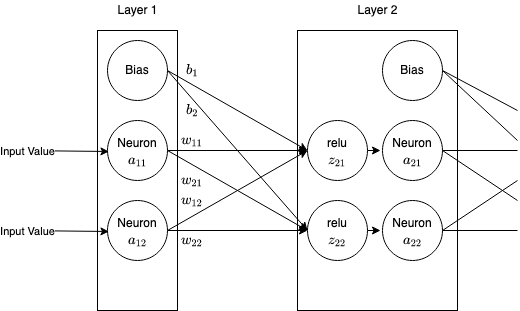
\includegraphics[width=0.6\textwidth]{two_neuron_network_1}
\end{figure}

\begin{equation}
    \begin{aligned}
        z_{21} &= a_{11}w_{11} + a_{12}w_{12} + b_{1} \, \, \, \, \, \, \, z_{22} = a_{11}w_{21} + a_{12}w_{22} + b_{2} \\
        a_{21} &= relu(z_{21}) \, \, \, \, \, \, \, a_{22} = relu(z_{22}) 
    \end{aligned}
\end{equation}


As networks become larger using this notation above becomes cumbersome. So we
use matrices to simplify the situation. Where \(X\) is the input matrix, \(W\)
is the weights, \(B\) is the bias, \(activationFunc(x)\) is the activation function and finally \(A\) is the output activation.

\begin{equation}
    \begin{aligned}
        X = \begin{bmatrix}
            a_{11} \\
            a_{12}
        \end{bmatrix} \, \, \, \, \, \, \,
        W &= \begin{bmatrix}
            w_{11} & w_{12} \\
            w_{21} & w_{22}
        \end{bmatrix} \, \, \, \, \, \, \,
        B = \begin{bmatrix}
            b_{1} \\
            b_{2}
        \end{bmatrix} \\[10pt]
        A &= activationFunc( W^{T}X + B)
    \end{aligned}
\end{equation}

In my implementation there are only two layer types. Hidden layers and output
layers. The only difference between these two layers is the activation function
that they use. Hidden layers use the ReLU activation function which is a simple
piecewise non-linear function described as such:
\begin{equation}
    relu(z) = max(0,z)
\end{equation}
This function has become the de facto application function in dense hidden
layers since its debut in 2011. \cite{glorot2011deep}. In Elixir the forward
action in the hidden layer is implemented like so: \footnote{The pipe operator
\lstinline{|>} transforms the function \lstinline{val_a |> a_function(val_b)}
into \lstinline{a_function(val_a, val_b)}}
\begin{lstlisting}
  def forward(previous_activation, weights, bias) do
    weights|> Matrex.transpose()
    |> Matrex.dot(previous_activation)
    |> Matrex.add(bias)
    |> relu()
  end

  defp relu(z_vector) do
    z_vector|> Matrex.apply(
        fn value, _index -> if value > 0, do: value, else: 0 end
    )
  end
\end{lstlisting}

The output layer uses a more complex activation function, the softmax function,
which transforms its inputs into probabilities. The sum of these probabilities
is always 1. This is the softmax function, where \(z\) is a \(i \times 1\)
vector:
\begin{equation}
    softmax(z)_{i} = \frac{e^{z_{i}}}{\sum_{j=1}^{n} e^{z_{j}}}
\end{equation}

This function is implemented the categorical output layer like so:
\begin{lstlisting}
    def forward(previous_activation, weights, bias) do
        weights|> Matrex.transpose()
        |> Matrex.dot(previous_activation)
        |> Matrex.add(bias)
        |> softmax()
    end

    defp softmax(z_vector) do
        stabilised_vec = Matrex.subtract(z_vector, Matrex.max(z_vector))
        exp = Matrex.apply(stabilised_vec, :exp)
        Matrex.divide(exp, Matrex.sum(exp))
    end
\end{lstlisting}

% show forward propagation function across the networks





% put equations here

% second diagram here
% second equations here

% $$a_{2} = relu(z)$$

% $$z = a_{1}w + b$$

% \begin{figure}[h]
%     \centering
%     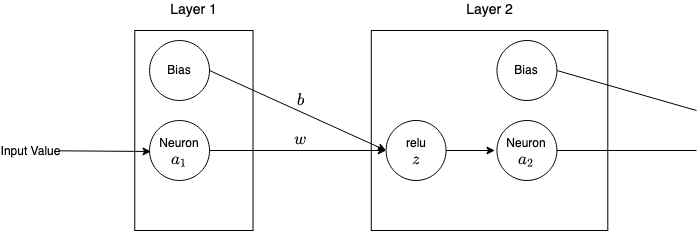
\includegraphics[width=0.6\textwidth]{simplest_neural_network_1}
% \end{figure}
% \begin{equation}
%     z_{21} = a_{11}w_{11} + a_{12}w_{12} + b_{1} \, \, \, \, \, \, \, z_{22} = a_{11}w_{21} + a_{12}w_{22} + b_{2}
% \end{equation}
% \begin{equation}
%     a_{21} = relu(z_{21}) \, \, \, \, \, \, \, a_{22} = relu(z_{22}) 
% \end{equation} 
% \begin{equation}
%     z = a_{1}w + b
% \end{equation}
% \begin{equation}
%     a_{2} = relu(z)
% \end{equation}

% The activation function being used
% in the hidden layers in this project is the ReLU function, which has become the de
% facto activation function since its discovery in 2011. \cite{glorot2011deep}

% %-----------------------------------------------------------------------------------------
\section{Reflection}
%-----------------------------------------------------------------------------------------
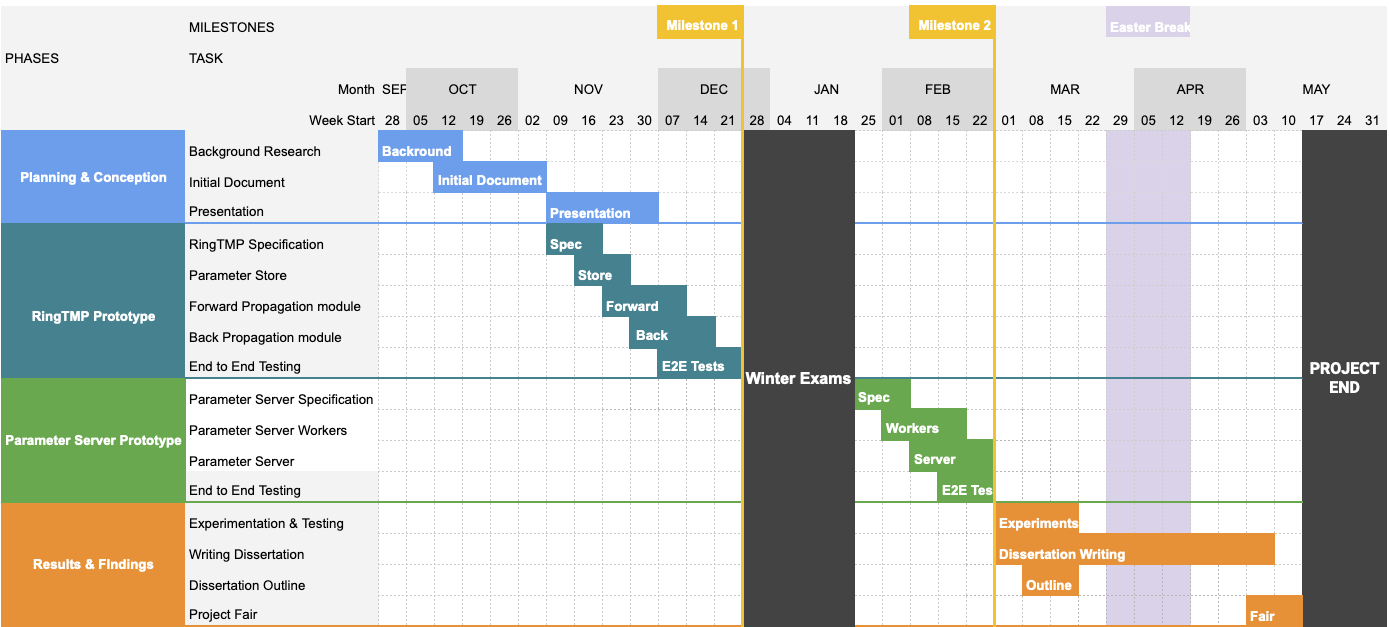
\includegraphics[width=16cm, height=8cm]{BetterGant.png}
Overall the project as gone adequately. I found it difficult to stick to the
timeline as it was hard to judge what parts of the project would take a long or
short amount of time. It took until just before christmas to understand the
mathematics of the neural network and create it. It underpinned my whole project
so it was very important it functioned correctly, so I spent much time with
rigorous testing. While I enjoyed creating it, it was far too time consuming and
looking back I should have used an already available neural networking library.
Distributing the took far less time than I expected, with elixir it was much
easier to distribute the network across different nodes. Especially for the
parameter server which took a matter of days to make. I think I achieved most of
the aims I set out to. While I couldn't observer
% %-----------------------------------------------------------------------------------------
\section{Future Work }
%-----------------------------------------------------------------------------------------
\lipsum[5-7]
% %-----------------------------------------------------------------------------------------
\section{Conclusion}
%-----------------------------------------------------------------------------------------
In conclusion machine learning algorithms already power large parts of our
digital lives. This is driven by data hungry learning models with potentially
billions of parameters. However now so much data is being produced that it is no
longer viable to centralise the data, leading to the need for efficient machine
learning on-device and communication between devices to improve the model. I
have introduced a new machine learning paradigm that should be more power
efficient than existing frameworks on low power devices over a local network. I
have displayed and explained the relevant research in distributed machine
learning and related fields, as well as core machine learning and neural
networking concepts. I have also shown the project timeline of building the new
framework, my testing methodology and how I will control risk within my project.


%-----------------------------------------------------------------------------------------

\clearpage
% \bibliographystyle{ieeetr}
\bibliographystyle{unsrt}

\bibliography{References/references}

\clearpage
\begin{appendices}
\section{Appendix 1}
\subsubsection{Code Listings}
\begin{lstlisting}[caption={Network Initialisation}, label={network_initialisation}]
defmodule FeedForwardNetwork.DefineNetwork
  defp initialise_parameters(definition, initial_seed) do
    definition
    |> Enum.reduce(
      {[], initial_seed},
      fn layer, {acc, seed_state} ->
        {layer, new_state} = initialise_layer(layer, seed_state)
        {acc ++ [layer], new_state}
      end
    )
  end

  defp initialise_layer({layer_type, input_size, output_size}, seed_state) do
    init_type = layer_to_init(layer_type)

    {initial_weights, seed_state} =
      initialise_weights(input_size, output_size, init_type, seed_state)

    initial_bias = initialise_bias(output_size)

    {{layer_type, initial_weights, initial_bias}, seed_state}
  end

  defp initialise_weights(col, row, init_type, seed_state) do
    {_, _, _, seed_state, list_of_lists} =
      Enum.reduce(
        0..(col - 1),
        {row, col, init_type, seed_state, []},
        &random_row/2
      )
    {Matrex.new(list_of_lists), seed_state}
  end

  defp random_row(_x, {row, col, init_type, seed_state, acc}) do
    {_, _, new_state, row_vals} =
      Enum.reduce(
        0..(row - 1),
        {col, init_type, seed_state, []},
        &random_val/2
      )
    {row, col, init_type, new_state, [row_vals | acc]}
  end

  defp random_val(_x, {n, :he, seed_state, acc}) do
    {val, new_state} = :rand.normal_s(0, 2 / n, seed_state)
    {n, :he, new_state, [val | acc]}
  end

  defp random_val(_x, {col, :pos, seed_state, acc}) do
    {val, new_state} = :rand.normal_s(0.5, 0.25, seed_state)
    {col, :pos, new_state, [val | acc]}
  end

  defp random_val(_x, {n, :xavier, seed_state, acc}) do
    {val, new_state} = :rand.normal_s(0, 1 / n, seed_state)
    {n, :xavier, new_state, [val | acc]}
  end

  defp initialise_bias(col) do
    Matrex.zeros(col, 1)
  end

  defp layer_to_init(:hidden_layer), do: :pos
  defp layer_to_init(:output_layer), do: :xavier
end
\end{lstlisting}

\begin{lstlisting}[caption={Cost Function}, label={cost_function}]
  def loss(activation, target_activation) do
    target_position = get_target_category(target_activation)

    activation
    |> Matrex.at(target_position, 1)
    |> (fn x ->
          if x == 0.0, do: 100, else: -:math.log(x) end
        end).()
  end

  defp get_target_category(target_activation) do
    {row, _col} = Matrex.size(target_activation)

    Enum.map(1..row, fn x -> [x] end)
    |> Matrex.new()
    |> Matrex.multiply(target_activation)
    |> Matrex.sum()
    |> round()
  end
\end{lstlisting}

\section{two}


\end{appendices}
\end{document}
